% Generated by extension/synthesis/make_assets.py. Do not edit.
\definecolor{propcol}{HTML}{217D91}
\definecolor{pairedcol}{HTML}{5D6670}
\definecolor{semicol}{HTML}{C9803A}
\definecolor{champcol}{HTML}{8E4B8C}
\definecolor{ridgecol}{HTML}{9AA3AB}
\definecolor{meancol}{HTML}{A64442}
\definecolor{sitecol}{HTML}{6A8FB3}
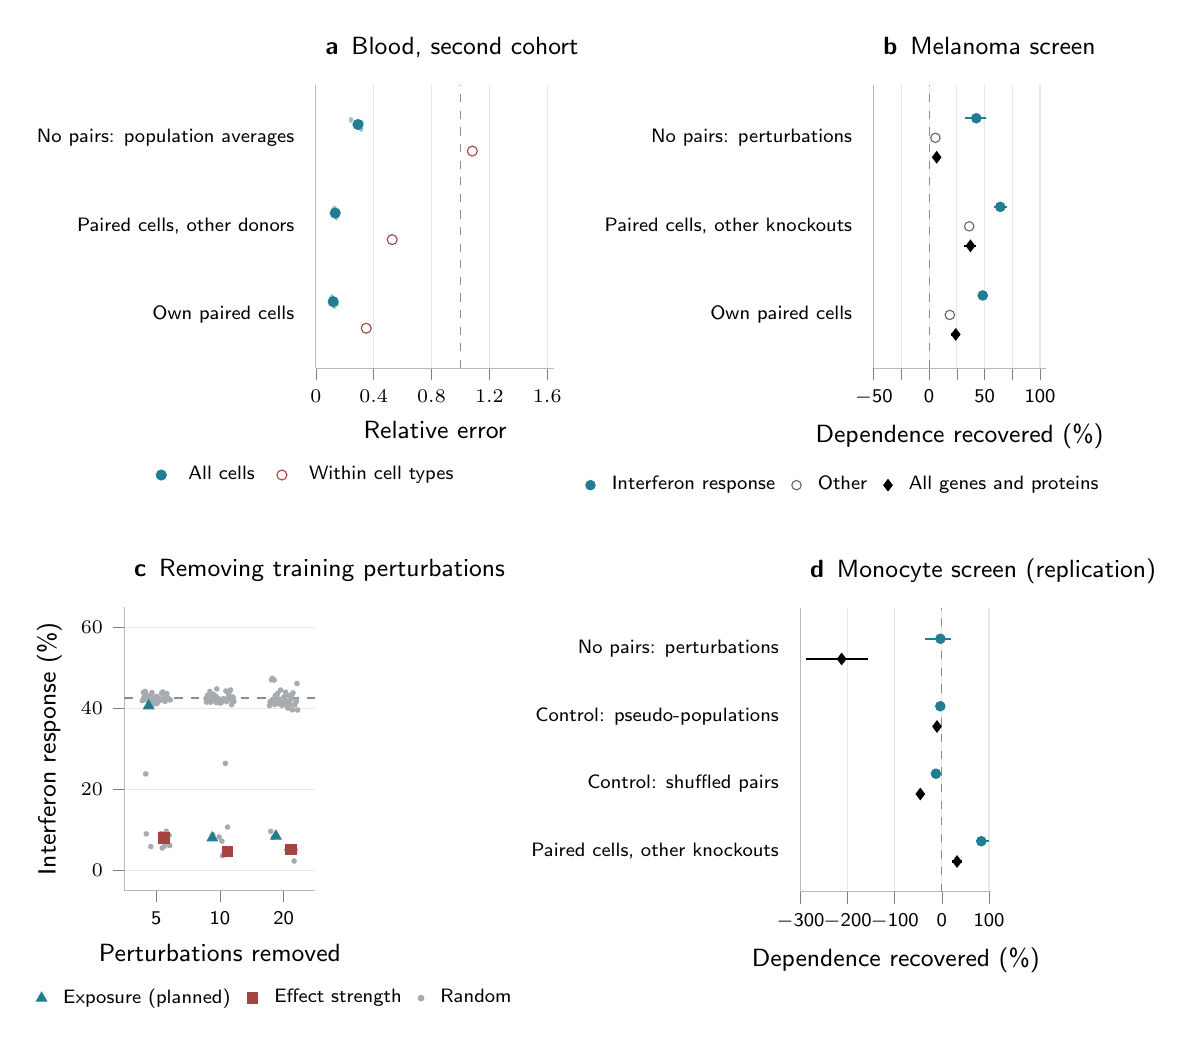
\begin{tikzpicture}[font=\sffamily]
\begin{axis}[name=a,scale only axis,width=.25\textwidth,height=3.6cm,xmin=0,xmax=1.65,
 ymin=.4,ymax=3.6,xtick={0,.4,.8,1.2,1.6},ytick={1,2,3},
 yticklabels={{Own paired cells},{Paired cells, other donors},{No pairs: population averages}},
 xlabel={Relative error},
 title={\textbf{a}\enspace Blood, second cohort},
 axis x line*=bottom,axis y line*=left,tick align=outside,xmajorgrids=true,grid style={gray!18},axis line style={gray!55},tick label style={font=\sffamily\scriptsize},label style={font=\sffamily\small},clip=false,title style={font=\sffamily\small,at={(0,1)},anchor=base west,yshift=5pt},y tick style={draw=none}]
\draw[dashed,black!45] (axis cs:1,.4) -- (axis cs:1,3.6);
\addplot[only marks,mark=*,mark size=.6pt,color=propcol!45] coordinates { (0.1282,1.090) (0.1256,1.107) (0.1467,1.124) (0.1235,1.141) (0.1057,1.159) (0.1105,1.176) (0.1095,1.193) (0.1112,1.210) };
\addplot[only marks,mark=*,mark size=.6pt,color=propcol!45] coordinates { (0.1424,2.090) (0.1377,2.107) (0.1383,2.124) (0.1401,2.141) (0.1385,2.159) (0.1271,2.176) (0.1203,2.193) (0.1295,2.210) };
\addplot[only marks,mark=*,mark size=.6pt,color=propcol!45] coordinates { (0.3142,3.090) (0.3108,3.107) (0.3052,3.124) (0.3030,3.141) (0.2952,3.159) (0.3175,3.176) (0.2438,3.193) (0.2433,3.210) };
\addplot[only marks,mark=*,mark size=1.8pt,color=propcol] coordinates { (0.1201,1.15) (0.1342,2.15) (0.2916,3.15) };
\addplot[only marks,mark=o,mark size=1.8pt,color=meancol] coordinates { (0.3485,0.85) (0.5280,1.85) (1.0820,2.85) };
\end{axis}
\begin{axis}[hide axis,scale only axis,width=1pt,height=1pt,xmin=0,xmax=1,ymin=0,ymax=1,at={(a.outer south)},anchor=north,yshift=-2pt,legend style={draw=none,font=\sffamily\scriptsize,at={(0.5,0.5)},anchor=north,legend columns=2,column sep=6pt,cells={anchor=west}}]
\addlegendimage{only marks,mark=*,mark size=1.8pt,color=propcol}
\addlegendentry{All cells}
\addlegendimage{only marks,mark=o,mark size=1.8pt,color=meancol}
\addlegendentry{Within cell types}
\end{axis}
\begin{axis}[at={(a.outer north east)},anchor=outer north west,xshift=.1cm,name=b,scale only axis,width=.18\textwidth,height=3.6cm,xmin=-50,xmax=105,
 ymin=.4,ymax=3.6,xtick={-50,-25,0,25,50,75,100},xticklabels={$-$50,,0,,50,,100},
 ytick={1,2,3},
 yticklabels={{Own paired cells},{Paired cells, other knockouts},{No pairs: perturbations}},
 xlabel={Dependence recovered (\%)},
 title={\textbf{b}\enspace Melanoma screen},
 axis x line*=bottom,axis y line*=left,tick align=outside,xmajorgrids=true,grid style={gray!18},axis line style={gray!55},tick label style={font=\sffamily\scriptsize},label style={font=\sffamily\small},clip=false,title style={font=\sffamily\small,at={(0,1)},anchor=base west,yshift=5pt},y tick style={draw=none}]
\draw[dashed,black!45] (axis cs:0,.4) -- (axis cs:0,3.6);
\draw[propcol,line width=.8pt] (axis cs:43.96,1.22) -- (axis cs:53.20,1.22);
\draw[black,line width=.8pt] (axis cs:19.80,0.78) -- (axis cs:27.75,0.78);
\draw[propcol,line width=.8pt] (axis cs:58.30,2.22) -- (axis cs:69.92,2.22);
\draw[black,line width=.8pt] (axis cs:31.65,1.78) -- (axis cs:42.22,1.78);
\draw[propcol,line width=.8pt] (axis cs:32.37,3.22) -- (axis cs:51.44,3.22);
\draw[black,line width=.8pt] (axis cs:4.05,2.78) -- (axis cs:9.42,2.78);
\addplot[only marks,mark=*,mark size=1.7pt,color=propcol] coordinates { (48.33,1.22) (64.17,2.22) (42.52,3.22) };
\addplot[only marks,mark=o,mark size=1.7pt,color=pairedcol] coordinates { (18.66,1) (36.17,2) (5.66,3) };
\addplot[only marks,mark=diamond*,mark size=2pt,color=black] coordinates { (24.00,0.78) (37.27,1.78) (6.79,2.78) };
\end{axis}
\begin{axis}[hide axis,scale only axis,width=1pt,height=1pt,xmin=0,xmax=1,ymin=0,ymax=1,at={(b.outer south east)},anchor=north east,yshift=-2pt,legend style={draw=none,font=\sffamily\scriptsize,at={(1,0.5)},anchor=north east,legend columns=3,column sep=4pt,cells={anchor=west}}]
\addlegendimage{only marks,mark=*,mark size=1.7pt,color=propcol}
\addlegendentry{Interferon response}
\addlegendimage{only marks,mark=o,mark size=1.7pt,color=pairedcol}
\addlegendentry{Other}
\addlegendimage{only marks,mark=diamond*,mark size=2pt,color=black}
\addlegendentry{All genes and proteins}
\end{axis}
\begin{axis}[at={(a.outer south west)},anchor=outer north west,yshift=-1.3cm,name=c,scale only axis,width=.2\textwidth,height=3.6cm,
 xmin=.5,xmax=3.5,ymin=-5,ymax=65,xtick={1,2,3},xticklabels={5,10,20},ytick={0,20,40,60},
 xlabel={Perturbations removed},ylabel={Interferon response (\%)},
 title={\textbf{c}\enspace Removing training perturbations},
 axis x line*=bottom,axis y line*=left,tick align=outside,ymajorgrids=true,grid style={gray!18},axis line style={gray!55},tick label style={font=\sffamily\scriptsize},label style={font=\sffamily\small},clip=false,title style={font=\sffamily\small,at={(0,1)},anchor=base west,yshift=5pt}]
\draw[dashed,black!45] (axis cs:.5,42.52) -- (axis cs:3.5,42.52);
\addplot[only marks,mark=*,mark size=.8pt,color=pairedcol!55] coordinates { (0.780,41.89) (0.789,41.97) (0.798,43.91) (0.807,42.70) (0.816,43.18) (0.825,44.17) (0.834,23.78) (0.843,8.97) (0.852,42.56) (0.861,43.22) (0.870,41.81) (0.879,42.07) (0.888,41.99) (0.897,42.11) (0.906,42.49) (0.915,5.84) (0.924,42.77) (0.933,43.87) (0.942,40.91) (0.951,41.93) (0.960,42.50) (0.969,42.40) (0.978,42.35) (0.987,42.30) (0.996,41.15) (1.004,42.92) (1.013,41.20) (1.022,41.98) (1.031,41.86) (1.040,42.51) (1.049,42.01) (1.058,42.12) (1.067,41.98) (1.076,9.05) (1.085,43.70) (1.094,5.48) (1.103,44.03) (1.112,42.17) (1.121,42.57) (1.130,5.98) (1.139,41.68) (1.148,42.23) (1.157,9.62) (1.166,43.60) (1.175,42.34) (1.184,42.23) (1.193,42.38) (1.202,8.63) (1.211,6.11) (1.220,42.05) (1.780,42.38) (1.789,41.52) (1.798,41.64) (1.807,43.21) (1.816,42.41) (1.825,41.84) (1.834,41.98) (1.843,44.16) (1.852,41.51) (1.861,42.83) (1.870,42.08) (1.879,42.27) (1.888,8.77) (1.897,43.45) (1.906,41.91) (1.915,42.65) (1.924,41.88) (1.933,42.99) (1.942,41.42) (1.951,44.77) (1.960,41.97) (1.969,42.42) (1.978,41.73) (1.987,8.21) (1.996,41.31) (2.004,42.09) (2.013,41.34) (2.022,41.44) (2.031,7.18) (2.040,3.57) (2.049,42.33) (2.058,3.99) (2.067,42.17) (2.076,42.25) (2.085,26.39) (2.094,44.25) (2.103,41.65) (2.112,41.97) (2.121,10.66) (2.130,42.42) (2.139,43.26) (2.148,44.02) (2.157,42.19) (2.166,44.51) (2.175,42.28) (2.184,40.88) (2.193,42.28) (2.202,42.78) (2.211,42.47) (2.220,41.68) (2.780,40.67) (2.789,41.63) (2.798,9.59) (2.807,47.01) (2.816,41.84) (2.825,47.38) (2.834,42.20) (2.843,8.12) (2.852,46.95) (2.861,40.91) (2.870,43.13) (2.879,42.04) (2.888,42.50) (2.897,42.04) (2.906,43.63) (2.915,42.27) (2.924,41.18) (2.933,42.23) (2.942,41.50) (2.951,44.49) (2.960,40.94) (2.969,41.28) (2.978,40.70) (2.987,41.40) (2.996,41.42) (3.004,42.79) (3.013,41.52) (3.022,41.06) (3.031,43.96) (3.040,41.85) (3.049,5.08) (3.058,40.88) (3.067,40.05) (3.076,43.17) (3.085,41.32) (3.094,41.54) (3.103,40.86) (3.112,42.68) (3.121,42.38) (3.130,43.27) (3.139,39.61) (3.148,43.79) (3.157,5.36) (3.166,2.27) (3.175,40.83) (3.184,5.06) (3.193,41.53) (3.202,41.88) (3.211,46.10) (3.220,39.56) };
\addplot[only marks,mark=triangle*,mark size=2.1pt,color=propcol] coordinates { (0.88,40.56) (1.88,7.98) (2.88,8.42) };
\addplot[only marks,mark=square*,mark size=1.9pt,color=meancol] coordinates { (1.12,7.90) (2.12,4.66) (3.12,5.12) };
\end{axis}
\begin{axis}[hide axis,scale only axis,width=1pt,height=1pt,xmin=0,xmax=1,ymin=0,ymax=1,at={(c.outer south west)},anchor=north west,yshift=-2pt,legend style={draw=none,font=\sffamily\scriptsize,at={(0,0.5)},anchor=north west,legend columns=3,column sep=4pt,cells={anchor=west}}]
\addlegendimage{only marks,mark=triangle*,mark size=2.1pt,color=propcol}
\addlegendentry{Exposure (planned)}
\addlegendimage{only marks,mark=square*,mark size=1.9pt,color=meancol}
\addlegendentry{Effect strength}
\addlegendimage{only marks,mark=*,mark size=1pt,color=pairedcol!55}
\addlegendentry{Random}
\end{axis}
\begin{axis}[at={(c.outer north east)},anchor=outer north west,xshift=.1cm,name=d,scale only axis,width=.2\textwidth,height=3.6cm,xmin=-300,xmax=105,
 ymin=.4,ymax=4.6,xtick={-300,-200,-100,0,100},xticklabels={$-$300,$-$200,$-$100,0,100},
 ytick={1,2,3,4},
 yticklabels={{Paired cells, other knockouts},{Control: shuffled pairs},{Control: pseudo-populations},{No pairs: perturbations}},
 xlabel={Dependence recovered (\%)},
 title={\textbf{d}\enspace Monocyte screen (replication)},
 axis x line*=bottom,axis y line*=left,tick align=outside,xmajorgrids=true,grid style={gray!18},axis line style={gray!55},tick label style={font=\sffamily\scriptsize},label style={font=\sffamily\small},clip=false,title style={font=\sffamily\small,at={(0,1)},anchor=base west,yshift=5pt},y tick style={draw=none}]
\draw[dashed,black!45] (axis cs:0,.4) -- (axis cs:0,4.6);
\draw[black,line width=.8pt] (axis cs:20.70,0.85) -- (axis cs:43.08,0.85);
\draw[propcol,line width=.8pt] (axis cs:72.71,1.15) -- (axis cs:99.69,1.15);
\draw[black,line width=.8pt] (axis cs:-287.47,3.85) -- (axis cs:-157.29,3.85);
\draw[propcol,line width=.8pt] (axis cs:-35.65,4.15) -- (axis cs:19.48,4.15);
\addplot[only marks,mark=*,mark size=1.7pt,color=propcol] coordinates { (83.69,1.15) (-12.44,2.15) (-3.23,3.15) (-2.95,4.15) };
\addplot[only marks,mark=diamond*,mark size=2pt,color=black] coordinates { (32.37,0.85) (-45.59,1.85) (-10.24,2.85) (-212.41,3.85) };
\end{axis}
\end{tikzpicture}
